\section{Rise of Language Agents}

The previous sections have argued for the presence of intelligent behavior in \glspl{llm}, but their usage also introduces significant limitations and risks. One major concern is the high energy consumption required for training, which, when combined with uncurated data scraped from the internet, can reinforce harmful biases and discrimination in decision-making systems, such as those used for hiring \cite{parrots}. Additionally, since \glspl{llm} are trained on data up to a specific cutoff date, they lack awareness of information produced after that point and may perform poorly on topics with limited data, such as specialized fields. The phenomenon of generating factually incorrect or misleading outputs, commonly referred to as \textbf{hallucinations}, has also been well-documented \cite{bai2024hallucination}.

\pskip

To address these issues, ongoing research aims to mitigate harmful or undesirable outputs. One prominent approach is \gls{rlhf} (Reinforcement Learning with Human Feedback), where human users provide feedback on the quality of generated text, either through binary ratings or numerical scores. This feedback is used to train a neural network that serves as a reward function for the model or policy, in the language of \gls{rl}. The reward function then fine-tunes the policy to align the model with human values, such as promoting usefulness or avoiding harmful stereotypes \cite{ouyang2022traininglanguagemodelsfollow}.

\pskip

Another approach involves developing guardrails for \glspl{llm}’ outputs. These guardrails may include hard-coded rules, such as avoiding specific keywords, or use the model itself to critique its output based on predefined principles written in natural language \cite{dong2024buildingguardrailslargelanguage} \cite{yuan2024rigorllmresilientguardrailslarge}.

\pskip

The future trend in working with \glspl{llm} is shifting toward a more integrated approach in both academia and industry. As discussed, these models have exhibited behavior that increasingly aligns with our understanding of human intelligence. Their true potential lies in leveraging up-to-date knowledge bases while delegating specialized tasks to external tools, such as calculators or logical provers \cite{Trinh2024}. These tools can be easily integrated through text formats like \Gls{json}. When paired with a retrieval system, the rate of hallucinations in \glspl{llm} decreases significantly \cite{ding2024survey} \cite{wang2024evaluating}. 

\pskip

Given the intelligent behavior exhibited by \glspl{fm}, the trust they garner from users, and their ability to delegate specialized tasks, \glspl{fm} are poised to become the next widely adopted \Gls{ui}, much like the mouse and keyboard for personal computers or the touchscreen for handheld devices.

\begin{figure}[h!]
    \centering
    \captionsetup{format=plain, font=small, labelfont=bf}
    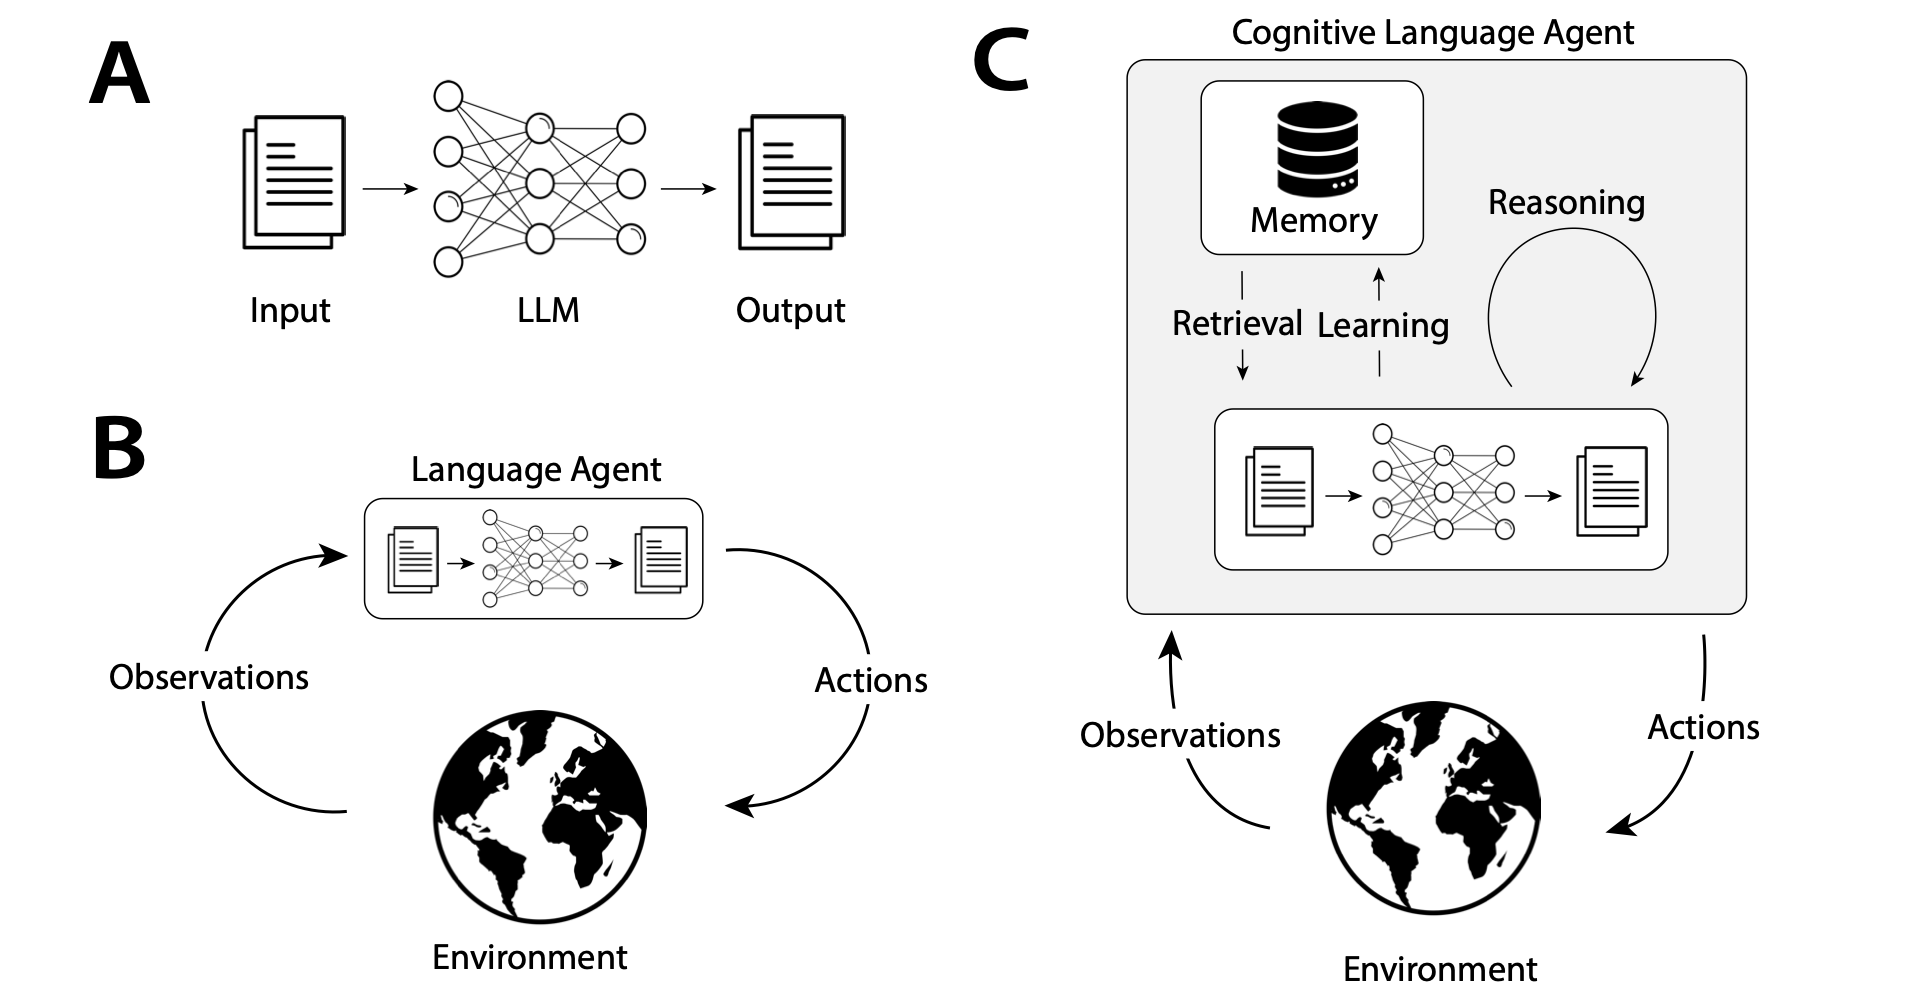
\includegraphics[width=\linewidth]{figures/cognitive_architectures.png}
    \caption[Illustration of Cognitive Architectures for Human Agents]{Reproduced from *Cognitive Architectures for Language Agents* by Sumers et al. \cite{sumers2024cognitivearchitectureslanguageagents}. The usage of \glspl{llm} is shifting towards human-aligned models (B) that interface with external tools to interact with an environment (C), rather than solely generating text as a response (A). The emergent abilities of large language models are increasingly being utilized to direct or delegate tasks to external systems, positioning them as intermediaries between computing systems and human users through the medium of natural language.}
    \label{fig:enter-label}
\end{figure}

\pskip

This idea has been echoed by Mei et al. \cite{aiasos}, who envision an operating system kernel responsible for system calls and process scheduling, paired with a language agent kernel that manages tasks such as context window management, information retrieval, and delegation to specialized language agents. In this framework, traditional programs expose a natural language interface, allowing programs to be controlled through natural language commands, with the \glspl{llm} kernel delegating user inputs accordingly.